\chapter{Background}

\section{Introduction to Fuzzing}

Fuzzing, or fuzz testing, is a software testing technique that includes feeding a huge amount of random data into the system, called SUT (System Under Test), to find unprecedented responses and reveal major programming errors, along with key security vulnerabilities. The primary objective of fuzzing is to identify vulnerabilities such as buffer overflows, memory leaks, and other security weaknesses that can be exploited by attackers.
\\The success of fuzzing is based on its capabilities for automatic test case generation and for focusing its attention on portions of programs that otherwise would not have been tested by other more traditional testing technique.
\\Indeed, it is particularly effective for applications with complex input grammars, where manual test case creation would be impracticable.

\subsection{Types of Fuzzing Techniques}
Fuzzing methodologies vary, and there exist a lot for different applications and purposes:

\begin{itemize}
    \item \textbf{Black-box Fuzzing}: This is a technique of generating inputs without prior knowledge of the internal structure of an application. It is easy to deploy but often less efficient as there is no internal feedback.
    
    \item \textbf{White-box Fuzzing}: This is one of those techniques that rely heavily on source code intuition, such as control flow and data flow, to provide maximum code coverage with test case generation. The approach often employs some sort of complex static and dynamic analysis methodologies.
    
    \item \textbf{Grey-box Fuzzing}: It's a strategy that combines the various merits of black-box and white-box fuzzing. It brings in partial knowledge about internal application details, and code coverage feedback guiding the generation of inputs. It balances simplicity with effectiveness, and an example might be the family of tools called AFL (American Fuzzy Lop).
\end{itemize}

\subsection{Fuzzing Inputs Generation}
There are also different ways to generate inputs for fuzzing:
\begin{itemize}
    \item \textbf{Mutation-based Fuzzing}: This generates new inputs through random mutations of existing inputs (for example modifying bits or bytes of existing test cases). It requires no knowledge about the structure of the inputs but is often a lot weaker compared with other generations for applications requiring highly structured inputs.
    
    \item \textbf{Generation-based Fuzzing}: This builds the inputs from scratch, based on a formal characterization of the input format, grammar or protocol specification. It has proved quite effective in applications where the inputs have to be complex or systematically structured.
\end{itemize}

\subsection{Coverage-Guided Fuzzing}
\textbf{Coverage-guided fuzzing} is a subtype of grey-box fuzzing that leverages code coverage information to drive the generation of test inputs. It aims to explore as many code paths as possible by continuously generating inputs that maximize the coverage.
\\For example, the American Fuzzy Lop (AFL) fuzzer is a popular coverage-guided fuzzer that uses a feedback loop to guide the generation of new test cases. AFL instruments the binary to track the code coverage during execution and uses this information to guide the mutation of test cases. The fuzzer maintains a queue of test cases and iteratively selects, mutates, and executes them to maximize the code coverage.
\\In this context is also important to describe the concept of \textbf{edge coverage}, that is a metric that measures the number of unique edges traversed by the program during execution. An edge is a transition between two basic blocks in the control flow graph of the program (a basic block is a sequence of instructions not containing any jumps or branches).
For example, consider the following code snippet:
\begin{lstlisting}
if (x > 0) {
    y = 1;
} else {
    y = 2;
}
\end{lstlisting}
In this case, there are two edges \ref{fig:sample_edge_graph}: one from the condition to the true branch and one from the condition to the false branch. The basic blocks are the condition, the true branch, and the false branch.
\\This edges are used in the \textbf{coverage map}, that is a binary compiled with edge coverage information, where each edge is mapped to a bit in the coverage map.
\begin{figure}[H]
    \centering
    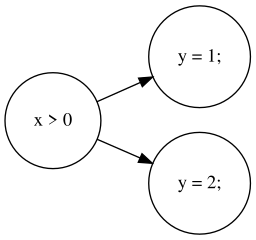
\includegraphics[width=0.5\textwidth]{Images/sample_edge_graph.png}
    \caption{Example of edge between basic blocks}
    \label{fig:sample_edge_graph}
\end{figure}
\phantom{}\\
When an edge is executed, the corresponding bit in the coverage map is set to a probability value. The fuzzer uses this information to guide the generation of new test cases that maximize the coverage.
\\Within this action a coverage-guided fuzzer maintains a \textbf{queue} of inputs and adds new inputs that had allowed it to increase the coverage of the program.
\\In particular, it adds to the queue those inputs that have allowed to increase the coverage of the program, and it uses a scheduler to select which input to mutate next.
\\The \textbf{scheduler} can be based on different strategies, such as the Coverage-Yield (CY) strategy, which uses a round-robin approach to select the next input to mutate, or the Outgoing Edges (OE) strategy, which prioritizes inputs that exercise new edges in the program (this is done by using metadata that keeps track of the outgoing edges of each state in the program and selecting the input that exercises the most new edges).
\\Talking about queue and inputs, we have to talk about corpus and how it is structured.
\\The \textbf{corpus} is a collection of inputs that the fuzzer uses to seed the initial test cases and to guide the mutation process.
The mix of corpus, coverage map, queue and scheduler is the core of the coverage-guided fuzzing strategy.
\\These are some examples of coverage-guided strategies:
\begin{itemize}
    \item \textbf{Multiple Corpus Single Map (MCSM)}: This strategy uses a single coverage map to track the coverage of the program and multiple queues to store the inputs. Each queue contains inputs that have allowed the fuzzer to reach a specific state of the program. The fuzzer uses a scheduler to select which input to mutate next based on the coverage achieved by the input.
    
    \item \textbf{Multiple Corpus Multiple Map (MCMM)}: This strategy uses multiple coverage maps to track the coverage of the program and multiple queues to store the inputs. Each queue contains inputs that have allowed the fuzzer to reach a specific state of the program. The fuzzer uses a scheduler to select which input to mutate next based on the coverage achieved by the input.
\end{itemize}

\section{Stateful Fuzzing: Concepts and Challenges}
\textit{Stateless fuzzing} is a traditional fuzzing technique that generates random inputs to test the behavior of an application. However, this approach is not always effective for applications that maintain internal states across multiple interactions.
\\For example cosidering an FTP server, like LightFTP, until the user is not authenticated, all the inputs are meaningless. In this case, the fuzzer should be able to generate a sequence of inputs that first authenticate the user and then test the behavior of the application.
\textit{Stateful fuzzing} adds state awareness to traditional fuzzing methods. It considers an application's internal state and how that state might affect subsequent inputs handling. This becomes particularly critical for applications that handle complex state information, such as network servers, databases, and interactive applications.

\subsection{Understanding Stateful Applications}
Stateful applications maintain state across multiple interactions or sessions. Examples include network servers that manage connection states, authentication states, session identifiers, or other state information specific to an application. These states significantly influence the processing of inputs and the behavior of the application over time.
\\Good practices in state transition management are crucial for both security and reliability: bugs related to state transitions can lead to vulnerabilities such as unauthorized access, denial of service (DoS), or data corruption. 
\\Stateful fuzzers attempt to model and explore these state transitions by generating input sequences that mimic valid usage scenarios while concurrently monitoring state changes to ensure comprehensive coverage of all possible transitions. To better understand this concept, consider a simple state model shown in Figure \ref{fig:simplestatemodel}.

\begin{figure}[h]
    \centering
    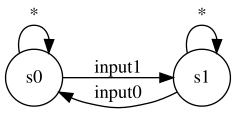
\includegraphics[width=0.5\textwidth]{Images/simplestatemodel.png}
    \caption{A simple state model illustrating state transitions in a stateful application}
    \label{fig:simplestatemodel}
\end{figure}


\subsection{Key Techniques in Stateful Fuzzing}
Stateful fuzzing involves several advanced techniques that distinguish it from traditional fuzzing approaches:

\begin{itemize}
    \item \textbf{State Modeling}: The process of building a model representing an application state machine by reverse engineering source code, observing real interactions, or guide test case generation in conjunction with machine learning techniques.
    
    \item \textbf{State Tracking}: This involves tracking the state of the application across successive inputs; indeed, tracking of network traffic, system calls, or internal state variables.
    
    \item \textbf{Feedback Mechanisms}: With feedback mechanisms, one can prioritize those test cases that tend to explore new states or code paths; hence, the general efficiency of fuzzing can be improved.
    
    \item \textbf{Sequence Generation}: It is the need to generate input sequences to properly model actual use, since the findings of vulnerabilities often depend on specific sequences or state transitions.
    
    \item \textbf{Learning-Based Approaches}: Certain fuzzers utilize machine learning or heuristic methodologies to dynamically ascertain the structural configuration of the application's state machine, thereby enabling the fuzzer to adjust and enhance its efficacy progressively.
\end{itemize}

\subsection{Challenges in Stateful Fuzzing}
Successfully performing testing is fraught with several challenges in stateful fuzzing:

\begin{itemize}
    \item \textbf{State Explosion}: As in real life, an application itself may have a number of possible states, and with more states, a risk for exponential growth in process complexity increases. In this case, state abstraction, pruning, or prioritization counters the \textit{state explosion} in an essential way.
    
    \item \textbf{Protocol Complexity}: Generating meaningful input sequences can involve deep knowledge of complex protocols or state machines. This often includes much domain-specific knowledge or even advanced algorithms.
    
    \item \textbf{Performance Overhead}: To date, state tracking performed by the application and input sequence generation can cause significant computational costs, hence slowing down the fuzzing process.

    \item \textbf{Handling Non-Deterministic Behavior}: The nondeterministic behavior of stateful applications often results from concurrency, differences in external inputs, or even timing variations. These factors therefore make the reproduction of bugs and receiving consistent fuzzing results usually difficult.

\end{itemize}

\section{Lighttpd: A Case Study for Stateful Fuzzing}
\textit{Lighttpd} is an open-source web server optimized for performance with very low memory usage. It is designed to handle huge volumes of parallel connections with minimal overhead, making it particularly useful on systems with limited resources or those requiring a high degree of concurrency. Its modular design and support for advanced web protocols make it a popular choice for embedded systems, cloud computing platforms, and high-traffic websites. It was used by popular websites like Wikimedia, YouTube, and SourceForge, nowadays is used in general for ...%TODO add more

\subsection{Overview of Lighttpd Architecture}
Lighttpd operates on an event-driven architecture, which enables it to serve many requests concurrently. An asynchronous I/O framework is employed to minimize overhead in network connections, allowing the server to scale efficiently under varying workloads. The key features of Lighttpd include:

\begin{itemize}
    \item \textbf{Modular Design}: Provides a series of modules for implementing functions like URL rewriting, HTTP compression, SSL/TLS, and WebSockets. The modular design allows for customization based on specific needs.
    
    \item \textbf{Protocol Support}: Out of the box, it supports HTTP/1.1, HTTPS, FastCGI, SCGI, and HTTP/2, making it suitable for a wide range of web applications and services.
    
    \item \textbf{Security Attributes}: Advanced integrated security features include TLS/SSL encryption, prevention of denial-of-service attacks, and multiple authentication options.
\end{itemize}

\subsection{Relevance of Lighttpd for Fuzzing}

Lighttpd is an important SUT for fuzzing due to its common use behind various internet applications.
These characteristics make it a suitable candidate for evaluating fuzzing techniques.
By default, Lighttpd is not stateful, but it maintains transient states during the processing of requests \ref{fig:lighttpdstatemodel}.
\begin{figure}[H]
    \centering
    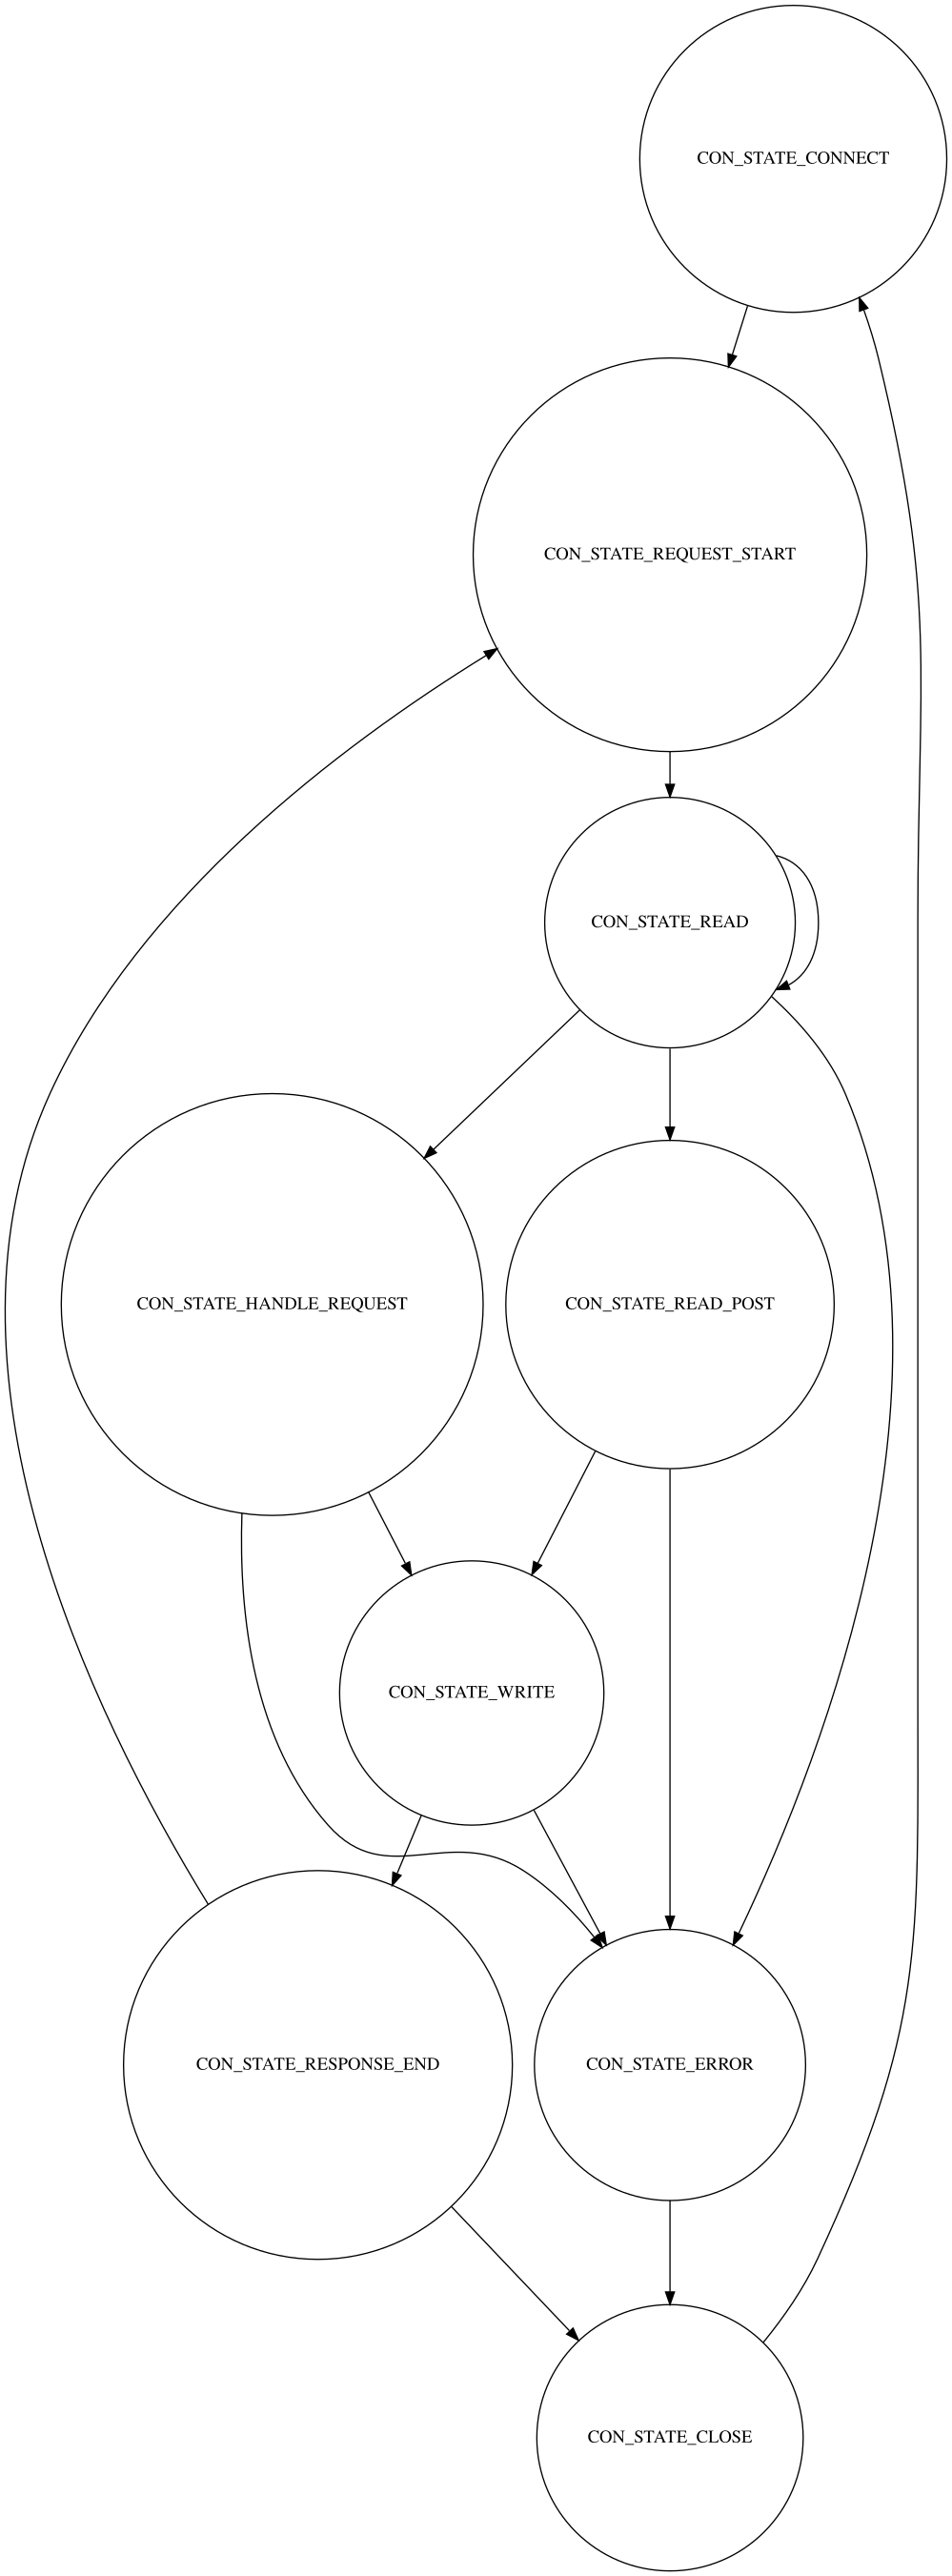
\includegraphics[width=0.6\textwidth]{Images/lighttpd_original.png}
    \caption{State model of Lighttpd}
    \label{fig:lighttpdstatemodel}
\end{figure}
\phantom{}\\
The state model seems to be complex, but the state are effectively transitory.
\\A sample flow of states in Lighttpd is as follows:
\begin{itemize}
    \item \textbf{CON\_STATE\_CONNECT}: The initial default state before a connection is established.
    
    \item \textbf{CON\_STATE\_REQUEST\_START}: The state right after a connection is established and wait for request.
    
    \item \textbf{CON\_STATE\_READ}: The state when the server is reading the request (here the server can be in a loop to read the request).
    
    \item \textbf{CON\_STATE\_HANDLE\_REQUEST}: The state when the server is processing the request, if body length is null.
    
    \item \textbf{CON\_STATE\_READ\_POST}: The state when the server is processing the request, if body length is more than 0.
    
    \item \textbf{CON\_STATE\_WRITE}: The state when the server is writing the response.
    
    \item \textbf{CON\_STATE\_REQUEST\_END}: The state after the request has been fully received.
    
    \item \textbf{CON\_STATE\_CLOSE}: The state when the connection is closed.
\end{itemize}
In the \textit{CON\_STATE\_CONNECT} we have no control of input, because it only changes when the connection is established.
\\The only stationary state could be the \textit{CON\_STATE\_READ}, because it is a loop that reads the request (i.e. if we send line by line the request, we will loop into it).
\\The other states are transitory because, at the end, we will go back to \textit{CON\_STATE\_REQUEST\_START} or \textit{CON\_STATE\_CONNECT}.
\\For this thesis, we have chosen to model the state of the server based on the existence or non-existence of a resources \ref{fig:existent_nonexistent_resource_statemodel}. A resource can be a file, a directory, or any other entity that can be accessed via HTTP. By considering two types of requests—those that attempt to access an existing resource and those that attempt to access a non-existing resource—we can effectively explore different states of the server.
\begin{figure}[H]
    \centering
    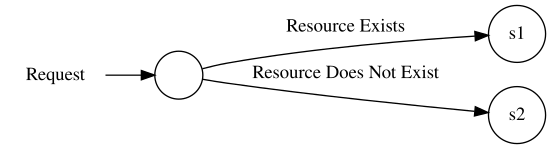
\includegraphics[width=0.8\textwidth]{Images/existent_nonexistent_resource.png}
    \caption{State model of Lighttpd based on the existence of resources}
    \label{fig:existent_nonexistent_resource_statemodel}
\end{figure}

\section{Fuzzers Overview: AFLNet, ChatAFL, and Fallaway}

For this thesis, three stateful fuzzers—AFLNet, ChatAFL, and Fallaway—will be benchmarked over Lighttpd.
 
% fare una pagina a testa
\subsection{AFLNet}
\textit{AFLNet} \cite{AFLNet} is a greybox fuzzer for protocol implementations. Unlike existing protocol fuzzers, it takes a mutational approach and uses statefeedback besides code-coverage feedback in order to guide the fuzzing process. AFLNet is seeded with a corpus of recorded message exchanges between the server and an actual client. No protocol specification or message grammars are required. It acts like a client, replaying variants of the original sequence of messages ever sent to the server, retaining only the variants which managed to increase the coverage of either code or state space. The response codes supplied by the server are utilised by AFLNet for server states that a message sequence manages to exercise. From this feedback, AFLNet identifies progressive regions in the state space and systematically steers towards such regions. 



\subsection{ChatAFL}
\textit{ChatAFL} \cite{chatafl} is a large language model-guided protocol fuzzer. It is based on AFLNet but integrates three concrete components. First, the fuzzer uses the LLM to extract a machine-readable grammar for a protocol that is used for structure-aware mutation. Second, the fuzzer uses the LLM to increase the diversity of messages in the recorded message sequences that are used as initial seeds. The fuzzer uses the LLM in an attempt to escape a coverage plateau, where LLM is prompted to generate messages to reach new states.
The ChatAFL artifact is configured within ProfuzzBench-a well-accepted benchmark for stateful fuzzing of network protocols. This way, this allows smooth integration with an already established format.



\subsection{Fallaway}
\textit{Fallaway} \cite{Fallaway} is a stateful, code coverage-based fuzzer and combines techniques from AFL* and AFLnet. It is implemented by extending the library LibAFL, which is a library to build modular fuzzers written in Rust. Its performance gain can partly be explained by the fact that the SUT process is reused for more than one test case. The state-awareness in test cases and feedback seems to have no effect on performance regarding code coverage. Nevertheless, there are a number of limitations in the approach followed by Fallaway which, after their resolution, might further increase the benefit that will be gained from having state-aware test cases and feedback.

